\documentclass{article}

\usepackage{graphicx}
\usepackage{listings}

\title{Homework 6}
\author{Mitchel Fields}
\begin{document}

\maketitle

\begin{tabular}{c | c}
$S_n$ & $S_{n+1}$\\ \hline
$S_0$ & $S_{1}$\\
$S_1$ & $S_{2}$\\
$S_2$ & $S_{0}$\\
$S_3$ & $S_{3}$
\end{tabular}

\begin{tabular}{c c | c c | c c | c c}
$n$ & & $n+1$ \\
$Q_n$ & $Q_{n+1}$ & $Q_n$ & $Q_{n+1}$ & $J_1$ & $K_1$ & $J_0$ & $K_0$ \\ \hline
0 & 0 & 0 & 1 & 0 & $\phi$ & 1 & $\phi$ \\
0 & 1 & 1 & 1 & 1 & $\phi$ & $\phi$ & 0 \\
1 & 1 & 0 & 0 & $\phi$ & 1 & $\phi$ & 1 \\
1 & 0 & 1 & 0 & $\phi$ & 0 & 0 & $\phi$
\end{tabular}

\noindent $J_1 = Q_1 + Q_0\\
K_1 = \overline{Q_1} + Q_0\\
J_0 = K_1\\
K_0 = Q_1 + \overline{Q_0}$

\begin{tabular}{c c | c c c}
$Q_n$ & $Q_{n+1}$ & $G$ & $Y$ & $R$ \\ \hline
0 & 0 & 0 & 0 & 1 \\
0 & 1 & 1 & 0 & 0 \\
1 & 1 & 0 & 1 & 0 \\
1 & 0 & 0 & 0 & 1
\end{tabular}

\noindent $G = \overline{Q_1}Q_0\\
Y = Q_1Q_0\\
R = \overline{Q_0}$\\

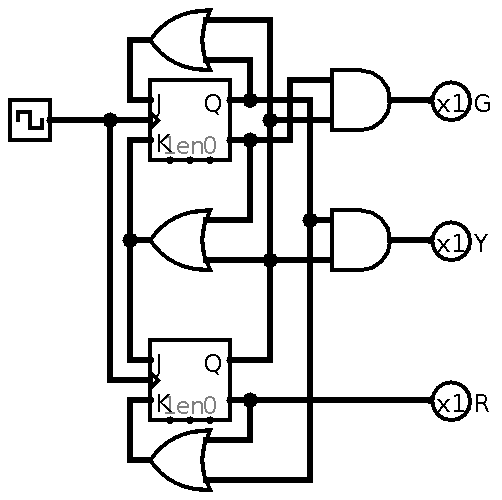
\includegraphics[scale=0.5]{hw6}

Python simulation:

\lstinputlisting[language=Python]{homework6.py}

\noindent 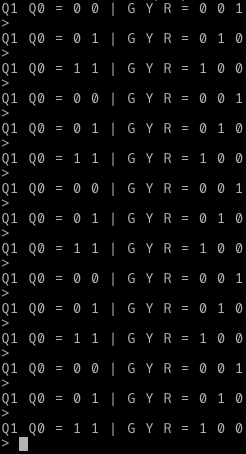
\includegraphics{hw6a}\\
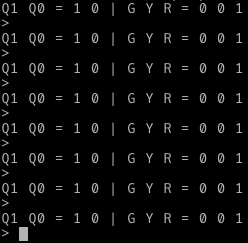
\includegraphics{hw6b}\\

\end{document}